% 
% Septiembre 2020
% Author: Mathieu Kessler
% Universidad Politécnica de Cartagena
% https://personas.upct.es/perfil/mathieu.kessler
% 
% 
\documentclass[9pt]{beamer}
\definecolor{links}{HTML}{2A1B81}
\hypersetup{colorlinks,linkcolor=,urlcolor=links}
 \usepackage[spanish]{babel}
\usepackage{colortbl}
\usepackage{graphicx}
\usepackage{amsmath,amssymb}
\usepackage{comma}
\usepackage{fancybox,color}
\usepackage[utf8]{inputenc}
\graphicspath{{../figures/}}
\setbeamertemplate{navigation symbols}{}
% -----------------------------------------------------------------------------
% To include multple images sequentially
% https://codeyarns.com/2010/02/09/how-to-do-image-animation-in-beamer/
% ------------------------------------------------------------------------------
 \usepackage{xmpmulti}
%------------------------------------------------------------------------------
\usepackage{xcolor}
\definecolor{mycodecolor}{rgb}{0.65,0.25,0.1}
\newcommand{\inlinecode}[1]{{\tt \textcolor{mycodecolor}{#1}}}
\usepackage{pythontex}
%--------------------
\usepackage{beamerthemeshadow}
\usepackage{xmpmulti}
\usepackage{mathtools}
\DeclarePairedDelimiter\abs{\lvert}{\rvert}%
\usepackage{tabularx}
\renewcommand\tabularxcolumn[1]{b{#1}}
\newcommand{\field}[1]{\mathbb{#1}}
\newcommand{\E}{\field{E}}
\newcommand{\R}{\field{R}}
\newcommand{\N}{\field{N}}
\newcommand{\Z}{\field{Z}}
\newcommand{\Q}{\field{Q}}
\newcommand{\EE}{\field{E}}
\newcommand{\FF}{\field{F}}
\newcommand{\GG}{\field{G}}
\renewcommand{\L}{\field{L}}
\renewcommand{\P}{\field{P}}
\newcommand{\LL}{{\mathfrak L}}

% define el folder donde del workspace, para cambiar inglés, ids,
% etc..
\newcommand{\workspacefolder}{stat\_labs }


\begin{document}
\title{Pandas: una introducción a la manipulación de datos con Python}

\author[Mathieu Kessler]{Mathieu Kessler}
\institute[]{Departamento de Matemática Aplicada y Estadística \\ Universidad Politécnica de Cartagena}
\date{@kessler\_mathieu}{}%{\href{https://code.visualstudio.com}{https://code.visualstudio.com}}
\titlegraphic{
\includegraphics[width=3cm]{1200px-Pandas_logo.svg.png}}

\begin{frame}
  \titlepage
\end{frame}

\begin{frame}[fragile]
  \frametitle{La librería pandas}
  \begin{block}{Qué es pandas}
    {\tt pandas} es una librería para el análisis de datos en Python, que fue desarrollada por Wes McKynney in 2008. Es uno de los proyectos apoyados por \href{https://numfocus.org}{NumFOCUS}, una asociación que fomenta proyectos y prácticas open source.\\
    Destaca por su gran riqueza de procedimientos para manipular y procesar datos, en particular datos con una componente temporal y su integración con numpy.
  \end{block}\onslide<2->

  Para usar {\tt pandas} en un programa o en un notebook, lo importamos con su alias.
  \begin{pyblock}
import pandas as pd
  \end{pyblock}
\end{frame}

\begin{frame}[fragile]
  \frametitle{Los dos objetos básicos en pandas}
  \begin{block}{Series y DataFrames}
    pandas define dos clases básicas
  \begin{itemize}
  \item \pyv{Series}: corresponden a vectores de datos.
  \begin{itemize}
  \item Es un vector unidimensional.
  \item  Tienen un ``índice'' ({\tt index}) que contiene etiquetas para cada dato. Las etiquetas no tienen por que ser únicas.
  \item Tienen opcionalmente un nombre ({\tt name}).
  \end{itemize}\onslide<2->
    \item \pyv{DataFrame}: Es una estructura 2D que contiene conjuntos de datos,
      \begin{itemize}
      \item Se puede pensar en una tabla bidimensional, donde  cada fila representa un individuo, cada columna es un \pyv{Series} que corresponde a una variable o característica del individuo.
      \item   Un \pyv{DataFrame} tiene un ``índice'' ({\tt index}) con etiquetas asociadas a cada individuo. Las etiquetas no tienen por qué ser únicas.
      \item Cada columna tiene un nombre.
      \item Podemos ver un {\tt DataFrame} como un {\tt dict} de {\tt Series}: las claves son los nombres de las columnas, sus valores son las {\tt Series}.
      \end{itemize}
  \end{itemize}
  \end{block}
\end{frame}
\begin{frame}[fragile]
  \frametitle{Pandas Series}
  La manera general de crear un Series es
  \begin{pyverbatim}
    pd.Series(data, index=None)
  \end{pyverbatim}
  \begin{itemize}
  \item   {\tt data} puede ser un vector o iterable (por ejemplo una lista), un \pyv{dict} o un valor escalar.
  \item Si no se proporciona un valor para \pyv{index}, se usarán enteros por defecto
  \item Admite el argumento opcional {\tt name}.
  \end{itemize}
  Ejemplos:
  \begin{pyblock}
s1 = pd.Series(
        [3, 2.5, -1],
        index=['a', 'b', 'c'],
        name='medición'
)
s2 = pd.Series(
        {'a': 3, 'b': 2.5, 'c': -1},
        name='medición'
)
  \end{pyblock}
\end{frame}
\begin{frame}[fragile]
 \frametitle{Índices en Pandas Series}
  Los {\tt index} son un concepto clave en {\tt Series} o \pyv{DataFrame}, en particular porque sirven para ``alinear'' las series cuando se combinan a través de operaciones, como sumas, restas, etc...
  \begin{pyconcode}
import pandas as pd
  \end{pyconcode}
  \begin{pyconsole}
s1 = pd.Series(
        [3, 2.5, -1],
        index=['a', 'b', 'c'],
)
s2 = pd.Series(
        [1, 0.5, 2],
        index=['b', 'c', 'd']
)
s1 + s2        
  \end{pyconsole}
\end{frame}
\begin{frame}[fragile]
  \frametitle{Índices en Pandas Series}
  Ejemplo con un índice duplicado: 
  \begin{pyconsole}
s1 = pd.Series(
        [3, 2.5, -1],
        index=['a', 'b', 'c'],
)
s2 = pd.Series(
        [1, 0.5, 2],
        index=['b', 'c', 'b']
)
s1 + s2        
  \end{pyconsole}
\end{frame}
\begin{frame}[fragile]
  \frametitle{Índices en Pandas Series}
 Y qué pasará en este caso, según vosotros?
  \begin{pyconsole}
s1 = pd.Series(
        [3, 2.5, -1, 10],
        index=['a', 'b', 'c', 'b'],
)
s2 = pd.Series(
        [1, 0.5, 2],
        index=['b', 'c', 'b']
)
s1 + s2        
  \end{pyconsole}
\end{frame}
\begin{frame}
  \frametitle{Pandas Series}
  Podéis encontrar en la referencia de la API de Pandas todos los atributos y métodos asociados a un {\tt Serie}: \href{https://pandas.pydata.org/pandas-docs/stable/reference/api/pandas.Series.html}{\pyv{pandas.Series}}
        \begin{center}
        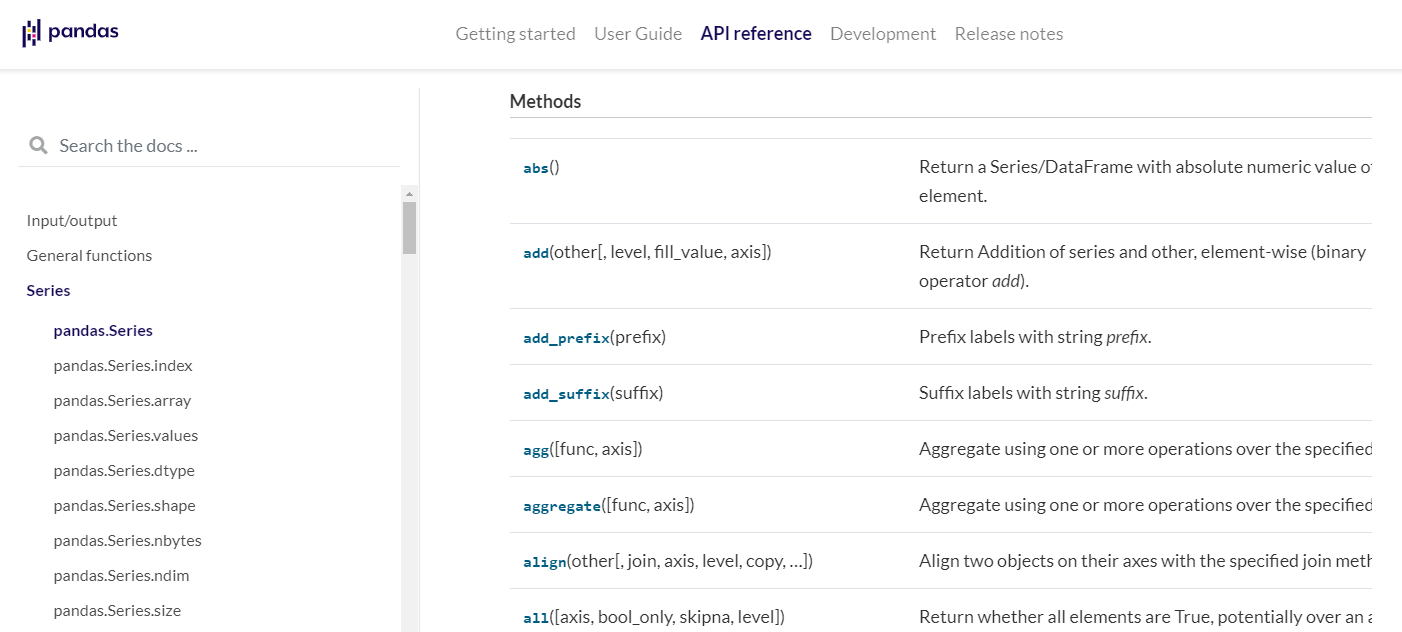
\includegraphics[width=11cm]{pandas_Series}
      \end{center}
\end{frame}
\begin{frame}[fragile]
  \frametitle{Métodos de Pandas Series}
  Estos métodos permiten aplicar una operación al conjunto de la Serie, sin tener que hacer un bucle recorriendo sus elementos.\\
  Por ejemplo:
  \begin{pyconsole}
s1 = pd.Series(
        [3, 2.5, -1, 2.5],
        index=['a', 'b', 'c', 'b'],
)
s1.sum()
  \end{pyconsole}
\pause  o
  \begin{pyconsole}
s1.drop_duplicates()
  \end{pyconsole}
  
\end{frame}
\begin{frame}[fragile]
  \frametitle{Pandas DataFrame}
  \begin{block}{La estructura de datos principal de pandas}
      La manera general de crear un DataFrame es
  \begin{pyverbatim}
    pd.DataFrame(data, index=None, columns=None)
  \end{pyverbatim}
  \end{block}
  \begin{itemize}
  \item   {\tt data} puede ser un array numpy, un iterable (por ejemplo una lista de listas), un \pyv{dict}.
  \item Si no se proporciona un valor para \pyv{index}, se usarán enteros por defecto
  \item El argumento \pyv{columns} indica las etiquetas para las columnas.
  \item data puede ser un \pyv{dict} donde las pares key:value son etiqueta:valores de cada columna.
  \end{itemize}\pause
{\footnotesize  Ejemplos:
  \begin{pyblock}
df1 = pd.DataFrame(
        [[3, 'r'],
         [2.5, 'g'],
         [-1, 'b']],
        index=['a', 'b', 'c'],
        columns=['x', 'color']
)
df2 = pd.DataFrame(
        {'x': [3, 2.5, -1],
         'color': ['r', 'g', 'b']},
        index=['a', 'b', 'c']
)
  \end{pyblock}
  }
\end{frame}
\begin{frame}[fragile]
  \frametitle{Pandas DataFrame}
  \pyv{data} también podría ser un \pyv{dict} de \pyv{Series}, lo que permite más flexibilidad con los índices: 
  \begin{pyconsole}
pd.DataFrame(
  {'x': pd.Series([3, 2.5, -1, 0], index=['a', 'b', 'c', 'd']),
   'color': pd.Series(['r', 'g', 'b'], index=['a', 'b', 'c'])}
)
  \end{pyconsole}
\end{frame}

\begin{frame}[fragile]
  \frametitle{Pandas DataFrame}
  \begin{block}{Métodos y atributos útiles con DataFrame}
    Si df es un pandas DataFrame
  \begin{pyverbatim}
# Métodos útiles para hacerse una idea del conjunto:
df.info()              # número de filas, columnas y tipo de datos
df.describe()          # resumen numérico de cada columna
df.head(7)             # las 7 primeras filas
df.tail(7)             # las 7 últimas filas
# Atributos útiles:
df.shape               # Dimensión del conjunto
df.columns             # etiquetas de las columnas
df.index               # etiquetas de las filas
df.values              # valores como ndarray de numpy
df.dtypes              # tipos de datos de cada columns
  \end{pyverbatim}
  \end{block}
\end{frame}
\begin{frame}[fragile]
  \frametitle{Leeremos siempre los datos desde una fuente externa}
  \begin{block}{Construir DataFrame}
    En todas las prácticas leeremos los datos desde una fuente externa.
    \begin{itemize}
    \item Desde un fichero local que nos habremos descargado 
    \item Desde un fichero situado en internet
    \item Desde una API de un servicio
    \end{itemize}
  \end{block}
  \pause
Para leer desde un archivo local, usaremos casi siempre \pyv{pd.read_csv}, que permite muchísima flexibilidad.\pause
\begin{block}{}
  \pyv{pd.read_csv} utiliza las primeras líneas del fichero para adivinar su estructura. Por ejemplo, infiere cómo están separados las columnas, si tiene cabecera, etc. Por lo tanto, en muchos casos, bastará con
  \begin{pyverbatim}
    pd.read_csv(<camino hasta el fichero de datos>)
  \end{pyverbatim}
  por ejemplo
  \begin{center}
  \begin{pyverbatim}
    pd.read_csv('data/datos.csv')
  \end{pyverbatim}
  \end{center}
\end{block}
 \end{frame}
\begin{frame}[fragile]
  \frametitle{Leeremos siempre los datos desde una fuente externa}
  \begin{block}{Parámetros más útiles de \pyv{pd.read_csv}}
    En el caso en que tuvieramos que especificar parámetros porque \pyv{pd.read_csv} no ha adivinado correctamente la estructura del fichero, éstos son útiles:
    \begin{itemize}
    \item \pyv{sep}: un \pyv{str} que contiene el caracter que delimita las columnas
    \item \pyv{skiprows}: un entero, número de filas que saltas al inicio del fichero. También puede ser una lista de los índices de filas.
    \item \pyv{encoding}: la codificación del fichero. Normalmente será 'utf-8', pero podría ser 'latin-1'.
    \item \pyv{thousands}: un \pyv{str} que contiene el caracter que separa los miles
    \item \pyv{dec}: un \pyv{str} que contiene el caracter que hace de separador decimal.
    \end{itemize}
  \end{block}
  \pause
Por ejemplo
\begin{block}{}
  \begin{pyverbatim}
df = pd.read_csv('data/datos.csv', sep = ';', skiprows = 3,
                                             encoding = 'latin-1')
  \end{pyverbatim}
\end{block}
 \end{frame}

\end{document}

  \begin{itemize}
  \item List \pyv{list}\\ \pause
    {\scriptsize
      \begin{minipage}{0.9\textwidth}
        \begin{block}{What is a list in Python?}
          A list is a collection of items. It is written as a list of
          comma-separated values between square brackets.\\
          The items can be of different types.\\
          Examples:\\
          \pyv{my_list = [3.21, 4.87, -9.22]}\\
          \pyv{my_list = ['stats', 23, True]}\\
          In a list, the items positions start from 0, and to access
          a given item, you can use square brackets.
          \begin{pyconsole}
my_list = ['stats', 12, True]
print(my_list[0])
          \end{pyconsole}
        \end{block}
      \end{minipage}}\pause
  \item Tuple \pyv{tuple}\\ \pause
    {\scriptsize
      \begin{minipage}{0.9\textwidth}
        \begin{block}{What is a tuple in Python?}
          A tuple is a collection of items. It is written as a list of
          comma-separated values between parenthesis.\\
          The items can be of different types.\\
          Examples:\\
          \pyv{my_tuple = (3.21, 4.87, -9.22)}\\
          \pyv{my_tuple = ('stats', 23, True)}\\
          The difference with a list is that a tuple is ``immutable'',
          which means that you cannot change an item of a tuple.\\
          Items in a tuple are acessed in a similar way as for a list.
        \end{block}
      \end{minipage}}
  \end{itemize}
\end{frame}
\begin{frame}[fragile]
  \frametitle{Basic data structures that we will use}
  \begin{itemize}
  \item Set \pyv{set}\\ \pause
    {\scriptsize
      \begin{minipage}{0.9\textwidth}
        \begin{block}{What is a set in Python?}
          A set us a collection of items with no duplicate elements. It is written as a list of
          comma-separated values between curly brackets.\\
          The items can be of different types. Sets are used to
          perform operations like union, intersection, difference, etc...
           Examples:\\           \pyv{fruits = {'apple',  'limon', 'banana'}}\\
               \pyv{vegetables = {'tomato', 'carrot', 'aubergine'}}
%           \pyv{vegetables = {'tomato', 'carrot', 'aubergine'}]
        \end{block}
      \end{minipage}}\pause
  \item Dictionaries \pyv{dict}\\ \pause
    {\scriptsize
      \begin{minipage}{0.9\textwidth}
        \begin{block}{What is a dictionary in Python?}
          A dictionary is collection which is indexed, its items are
          of the form key:value. Elements of an dictionary can be
          accessed through their indexes. Dictionaries are written with
          curly brackets.\\
          The items can be of different types.
          Examples:\\ \pyv{ages = {'john': 32,  'jane': 28, 'jim': 48}}\\
          You can access the value of an item, by indexing it using
          its key:
          \begin{pyconsole}
ages = {'john': 32,  'jane': 28, 'jim': 48}
print(ages['jane'])
\end{pyconsole}
        \end{block}
      \end{minipage}}
  \end{itemize}
\end{frame}
\begin{frame}[fragile]
  \frametitle{Basic input and output to and from the console}
  \begin{itemize}
  \item \pyv{print} is the basic command to display objects. \\
    You can print strings:\\
    \begin{pyconsole}
print('Hello world!')
    \end{pyconsole}
    \pause
    but also other objects
    \begin{pyconsole}
ages = {'john': 32,  'jane': 28, 'jim': 48}
print(ages)
    \end{pyconsole}
  \item<3-> To get data from the user in the console, the command is
    \pyv{input}.
    \begin{pyverbatim}
>>> n = input('Maximum number of cases:')      
\end{pyverbatim}
\begin{pycode}
n = 4
\end{pycode}
\pause
Take into account that the input variable value is a string. You may
need to turn  it to an integer or float for later use:
\begin{pyverbatim}
>>> print(int(n) + 6)
\end{pyverbatim}
  \end{itemize}
\end{frame}
\begin{frame}[fragile]
  \frametitle{Looping in Python}
  \begin{block}{The \pyv{for} command}
    The \pyv{for} command in Python allows to iterate over the elements
    of an object and executes at each iteration a series of
    instructions.
  \end{block}\pause
  \begin{itemize}
  \item The instructions to be iterated are written
    in an indented block under the \pyv{for} command:\\
    \begin{pyverbatim}
for ciudad in ['Madrid', 'Murcia', 'Cartagena']:
    print(ciudad)
  \end{pyverbatim}
  \pause
 Another example:\smallskip
 \begin{pyblock}
final_sum = 0
for i in (0, 1, 2, 3, 4, 5, 6):
    j = i * 2
    final_sum += j
print('The final result is: ' + str(final_sum))
\end{pyblock}
\pause
  \begin{block}{Notes}
    \begin{itemize}
    \item To express the sequence 0, 1, 2, 3, 4, 5, 6, we can use
      \pyv{range(6)}.    
      \item The operator \pyv{+=} indicates inplace increment, i.e
        \pyv{final_sum += j} is exactly the same as
        \pyv{final_sum = final_sum + j}
      \item The \pyv{+} operator for two strings performs
        concatenation. To use it, we had to first convert
        \pyv{final_sum} into a string. 
    \end{itemize}
  \end{block}
  \end{itemize}
\end{frame}
\begin{frame}[fragile]
  \frametitle{Exercices}
  \begin{enumerate}
    \item Write a program in a file called {\tt exercise-1-1.py} that
      requests an integer \pyv{n} from the user and prints the sum of
      the first \pyv{n} terms of the sequence $4$, $-4/3$, $4/5$, $-4/7
      \ldots$, i.e. the sequence
      $$ 4\times \frac{(-1)^{i}}{2\cdot i + 1},\ i = 0, 1, 2, \ldots$$
      \begin{itemize}
      \item \textit{Hint1: the power operator in Python is
          \pyv{**}.}
      \item \textit{Hint2: remember to use \pyv{int(n)} to transform the string
      input into an integer.}
      \end{itemize}
      Try your program with large or very large values of $n$.
    \item Write a program in a file called {\tt exercise-1-2.py} that
      requests an integer \pyv{n} from the user and prints the
      multiplication table of $n$. 
    \item Write a program in a file {\tt exercise-1-3.py} that prints the following pattern:
      \begin{center}
        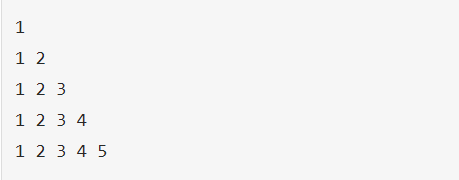
\includegraphics[width=5cm]{for_exercises_01}
      \end{center}
    \end{enumerate}  
  \end{frame}
  \begin{frame}[fragile]
    \frametitle{The conditional statements}
    \begin{block}{The \pyv{if}, \pyv{if ... else},
        \pyv{if ... else ... elif} commands}
    The \pyv{if} command in Python is an instruction that allows to
    trigger actions (instructions) based on whether a condition holds
    or not.
  \end{block}
  \pause
  \begin{itemize}
  \item   The structure of an \pyv{if} statement is similar to a
    \pyv{for} loop, the instructions to be executed in the case when
    the condition holds are collected in an indented block under the
    if clause.
    \begin{pyverbatim}
import math
n_string = input('Enter an positive integer ')
n = int(n_string)
if (n > 0):
    print('The square root of ' + str(n) + ' is ' + str(math.sqrt(n)))
  \end{pyverbatim}
\end{itemize}
\pause
\begin{block}{Note}
  The instruction \pyv{import math} imports the \pyv{math} module,
  which contains hundreds of relevant mathematical functions. Once
  we import the module, all its functions are available to us. To call a
  function from the \pyv{math} module, we need to prepend it with the
  name of the module it belongs to, in that case \pyv{math}. (More on
  modules later)
  
\end{block}
\end{frame}
\begin{frame}
  \frametitle{Exercices}
  \begin{enumerate}
  \item Write a program in a file called {\tt exercise-1-4.py} that
    requests an integer \pyv{n} from the user and checks whether $n$
    is a prime number
  \end{enumerate}  
\end{frame}
\begin{frame}[fragile]
  \frametitle{Functions}
  \begin{overlayarea}{\textwidth}{\textheight}
  \begin{block}{}
    Functions allow to encapsulate series of instructions, and
    call them easily with a single command (the function's name)
  \end{block}
  \pause
  \begin{itemize}
  \item \pyv{def} is the command used to define a function. 
  \item As usual, the list of instructions to be executed when the
    function is called is located in an indented block.
  \item The function admits arguments
  \item The \pyv{return} command is used to return a value (any Python object)
  \end{itemize}\pause
  Example:\vspace{-0.5cm}
  \begin{center}
    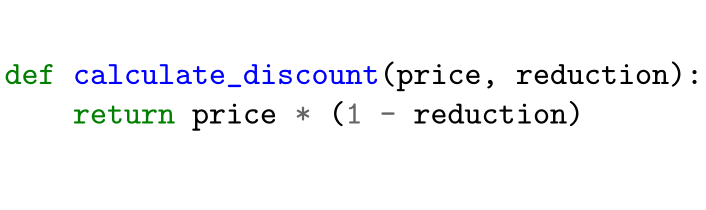
\includegraphics[width=7cm]{function_example}
  \end{center}\pause\vspace{-0.5cm}
  
You can then call the function in your program or at the console
prompt:
\pyv{calculate_discount(121, 0.2)} will return the discounted price.\pause
  \begin{block}{Use functions!}
    Using functions is a good practice, it improves the readability of
    your code and makes it easier to maintain or correct. 
  \end{block}
\end{overlayarea}
\end{frame}
\begin{frame}[fragile]
  \frametitle{Functions}
  \begin{block}{Recall the \pyv{calculate_discount} function:}
    \begin{pyverbatim}
def calculate_discount(price, reduction):
    return price * (1 - reduction)
  \end{pyverbatim}
  \end{block}
  \begin{itemize}
  \item<2->   When calling the function with \pyv{calculate_discount(121, 0.2)},
  Python uses the position of the provided values to assign them to
  the arguments.
  \begin{itemize}
  \item 121 is asigned to the argument \pyv{price}
  \item 0.2 is asigned to the argument \pyv{discount}
  \end{itemize}
\item<3-> The keywords for arguments can be used when calling the
  function. Their position is then irrelevant.
  \begin{pyverbatim}
calculate_discount(reduction=0.2, price=121) 
  \end{pyverbatim}
\item<4-> We must provide the correct number of values when calling the
  function, except if default values were specified for arguments in
  the function definition:
  \begin{pyverbatim}
def calculate_discount(price, reduction=0.2):
    return price * (1 - reduction)
  \end{pyverbatim}
  In that case, if the function is called with only one value, it will
  be assigned to the \pyv{price} argument and a default reduction of
  20\% will be applied.
  \end{itemize}
\end{frame}

\begin{frame}[fragile]
  \frametitle{Functions}
  \begin{block}{}
    Be kind to you and your users: document your code!
  \end{block}\pause
  \begin{itemize}
  \item<2->   Python uses Docstrings to provide information about the function. A
  docstring is a string that occurs as the first statement of a
  function (module, class, or method).
\item<3-> Dcstrings are surrounded by triple double quotes:
  \pyv{"""Here is the information text"""}
\item<4-> For simple cases, we can use one-line docstrings:
  {\footnotesize
  \begin{pyverbatim}
def calculate_discount(price, reduction):
    """Returns the discounted price, after applying reduction"""
    return price * (1 - reduction)
  \end{pyverbatim}
  }
\item<5-> This allows the user to get some information using \pyv{help}
  \begin{center}
    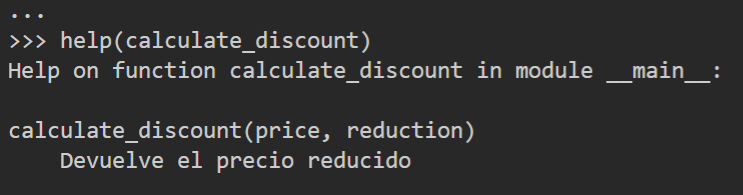
\includegraphics[width=8cm]{help_function_es}
  \end{center}

\end{itemize}
\end{frame}

\begin{frame}[fragile]
  \frametitle{Exercices}
  \begin{enumerate}
  \item As a continuation of {\tt exercise-1-3.py}, Write a function in a file called {\tt exercise-1-4.py} that
    takes an integer \pyv{n} as argument and returns \pyv{True} if
    \pyv{n} is a prime number and \pyv{False} otherwise.
  \item Add to the file {\tt exercise-1-4.py} code that requests an
    integer \pyv{n} from the user and prints out all the prime
    numbers less than \pyv{n}.
  \end{enumerate}  
\end{frame}

\begin{frame}[fragile]
  \frametitle{Using modules}
  \begin{block}{What is a module?}
    Modules are files with extension {\tt .py} which contain
    functions and objects (variables, classes, etc..) definitions. 
  \end{block}
  \begin{itemize}
  \item<2-> If I want to use the functions of a module, I need to
    import it. For example, assume I have created a file {\tt aux\_files.py} which
    collects all my useful functions, I will import it with:
    \begin{pyverbatim}
import aux_files
    \end{pyverbatim}
  \item<3-> Once that \pyv{aux_file} is imported, if I want to call
    its function \pyv{calculate_discount}, I will need to prepend the
    name of the module:
    \begin{pyverbatim}
import aux_files
discounted_price = aux_files.calculate_discount(121, 0.2)      
    \end{pyverbatim}
  \item<4-> To simplify the code, I can define a alias for a module
    when I import it:
        \begin{pyverbatim}
import aux_files as af
discounted_price = af.calculate_discount(121, 0.2)      
    \end{pyverbatim}
  \end{itemize}
\end{frame}

\begin{frame}[fragile]
  \frametitle{Using modules}
  \begin{itemize}
  \item<1-> I may import only one function or a few functions from a
    given module:
    \begin{pyverbatim}
from aux_files import calculate_discount
    \end{pyverbatim}
  \item<2-> In that case, there is no need to prepend the module's
    name when calling the function
    \begin{pyverbatim}
from aux_files import calculate_discount
discounted_price = calculate_discount(121, 0.2)      
    \end{pyverbatim}
  \item<3-> You may see in some code
        \begin{pyverbatim}
from aux_files import *
\end{pyverbatim}
That would allow to use any function of the module \pyv{aux_files} without
any need for prepending. This is a bad practice! It is recommended to
keep track explicitely of the module the function comes from.
  \end{itemize}
\end{frame}

\begin{frame}[fragile]
  \frametitle{Using modules}
  \begin{itemize}
  \item<1-> Python has a \textit{``Standard Library''} of useful modules that come
    with the Python installation. Moreover there are thousands of user
    contributed modules, prepared as \textit{``packages''} ready for
    download and installation.
  \item<2-> Modules from the \textit{``Standard Library''} can be
    imported directly from my code with the \pyv{import} command. For
    example the \pyv{math} module we mentioned earlier.
    \begin{pyverbatim}
import math
x = math.sin(0)
    \end{pyverbatim}
  \item<3-> To use third party modules, we should download the
    associated packages from repositories maintained by the
    community. 
  \item<4-> A very relevant one is {\tt \tt PyPI} \href{https://pypi.org/}{https://pypi.org/}, the Python Package Index, a huge
    repository of software developed and shared by the Python
    community. To download and install packages from {\tt PyPI}, we use
    the {\tt pip} utility. 
  \item<5-> Since we are using the Anaconda distribution, we won't use
    {\tt pip} and {\tt PyPI}, but the
    \href{https://anaconda.org/}{Anaconda Cloud} and the {\tt conda
      install} command.
  \end{itemize}
\end{frame}

\begin{frame}[fragile]
  \frametitle{Using external modules}
  \begin{itemize}
  \item We will make extensive use of some relevant modules for
    scientific computing, namely {\tt numpy}, {\tt scipy},
    {\tt matplotlib} and {\tt pandas}.
  \item<2-> If you have installed the full Anaconda distribution, all
    these modules are readily available, you can simply import them.
  \item<3-> If you have installed the miniconda distribution, you will
    have to prepare and use a virtual environment
    (see the document: ``Creating a virtual environment with
    conda''). In that case, the packages are retrieved and downloaded
    from the Anaconda Cloud repository and installed into your
    environment.
      \end{itemize} \onslide<4->
      \begin{block}{Importing {\tt numpy}}
        As an example, we will import {\tt numpy} using its
        conventional alias
        \begin{pyverbatim}
import numpy as np
x = np.arange(10)          
\end{pyverbatim}
We have used above the \pyv{arange} function from the numpy module,
that creates an array of equally spaced numbers, in that case,
integers ranging from 0 to 9.
\end{block}
\end{frame}

\begin{frame}[fragile]
  \frametitle{Functions, methods, attributes}
  \begin{block}{}
    Modules (almost) always define classes, which are templates for a
    relevant kind of objects for our program. For a given class, we
    define, 
    before hand, attributes and methods. The manipulation of objects
    of a given class is made much easier by using the class's
    attributes and methods.
  \end{block}
  \begin{itemize}
  \item<2-> An example of class in {\tt numpy} is its
    $N$-dimensional array, called {\tt ndarray}.
  \item<3-> In the previous code
        \begin{pyverbatim}
import numpy as np
x = np.arange(10)          
\end{pyverbatim}
{\tt x} is a {\tt ndarray}. You can check that with {\tt type(x)}.
\item<4-> There are many methods and attributes predefined for the
  {\tt ndarray} objects' class. Methods and attributes are applied to
  an object by appending them to the object's name after a dot.  Examples:
  \begin{itemize}
  \item<5-> \pyv{x.shape} is an attribute of \pyv{x}.
  \item<5-> \pyv{x.mean()} applies the \pyv{mean} method to \pyv{x}
  \end{itemize}
\item<6-> A method is like a function, but it always applies to an
  object. It may admit arguments, which are then indicated between the parenthesis.
  \end{itemize}
\end{frame}

\begin{frame}[fragile]
  \frametitle{Functions, methods, attributes}
  
  \begin{itemize}
  \item The \pyv{mean} only applies to a numpy array. The following
    code would throw an error:
    \begin{pyverbatim}
[0, 1, 2, 3, 4, 5, 6, 7, 8, 9].mean()      
    \end{pyverbatim}
  \item<2-> In order to list all methods and attributes available for
    an object, use \pyv{dir}:
    \begin{pyverbatim}
import numpy as np
x = np.arange(10)
print(dir(x))
\end{pyverbatim}
  \begin{center}
    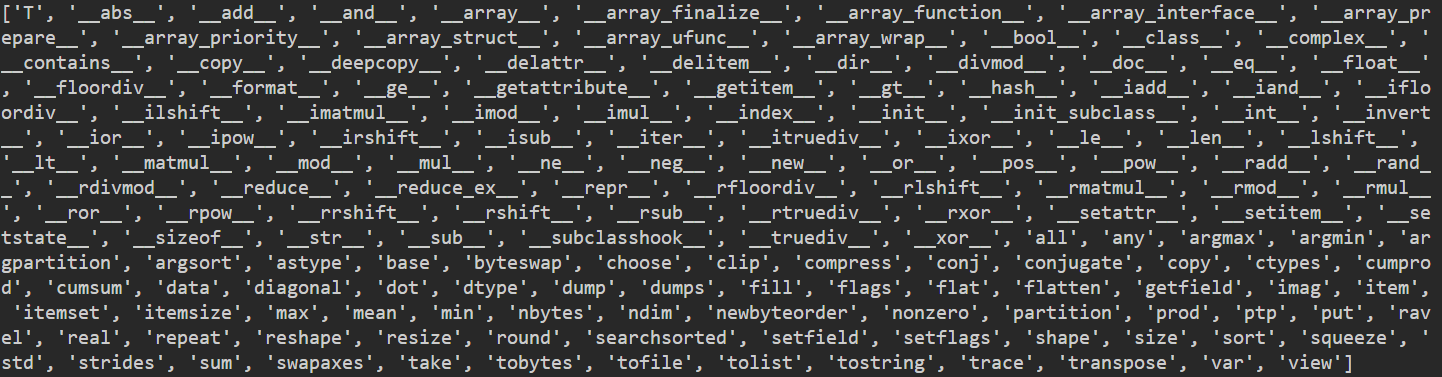
\includegraphics[width=10cm]{dir_ndarray}
  \end{center}
  The methods that begin and end with double ``\_'' are called
  ``dunder'' (double underscore)  methods and are for internal use of
  the module.
  \end{itemize}
\end{frame}

\begin{frame}[fragile]
  \frametitle{More on lists}
  We saw that, to access list items, we use indexing by position
  surrounded by square brackets.
{\footnotesize
  \begin{pyconsole}
my_list = ['data', 'science', 'analytics', 'statistics', 'mathematics']    
print(my_list[1])
\end{pyconsole}
}
\pause
\begin{block}{Slicing}
We often need to extract a number of consecutive items of a list. For
that purpose, we use \textit{slicing}, which takes the form:
\begin{pyverbatim}
my_list[start:stop:step]
\end{pyverbatim}
and extracts the items from the position {\tt start} to position {\tt
  stop} (excluding the position {\tt stop}), using a step of {\tt step}.
\begin{itemize}
\item<3-> If unspecified, the third argument {\tt step} takes the default value
  of 1.\\
  {\footnotesize
  \pyv{my_list[1:3]} will return \pyv{['science', 'analytics']}}
\item<4-> If unspecified, the {\tt start} argument has the default of
  0\\
  {\footnotesize 
    \pyv{my_list[:2]} will return \pyv{['data', 'science']}
    }
\item<5-> If you don't specify the {\tt stop} argument, the slice
  goes up to the end of the list.\\
  {\footnotesize
  \pyv{my_list[1:]} will return
  \pyv{['science', 'analytics', 'statistics', 'mathematics']}
  }
\end{itemize}
\end{block}
\end{frame}

\begin{frame}[fragile]
  \frametitle{Some operations on lists}
  \begin{block}{}
    Lists, together with dictionaries, are an essential data structure
    in Python. 
  \end{block}
  Some basic commands or methods:
    \begin{pyconsole}
my_list = [2, 1, -0.5, 0.287, 'abc']      
len(my_list) # returns the number of items
my_list[4] = 'cba' # changes the value of the item at position 4.
my_list
del my_list[2] # deletes item at position 2, modifies the list.
my_list
my_list.append('joe') # appends, modifies the list.
my_list
my_list.insert(1, 9.2) # inserts at position 1, modifies the list.
my_list
\end{pyconsole}

\end{frame}

\begin{frame}[fragile]
  \frametitle{How to make a copy of a list}
  \begin{block}{}
  To make a copy of a list, one could think of using a simple ``=''
  asignation operator:
  \begin{pyconsole}
my_duplicate = my_list
\end{pyconsole}
\pyconc[copy0]{my_list = [2, 1, -0.5, 0.287, 'abc']}
\pyconc[copy0]{my_duplicate = my_list}
\begin{pyconsole}[copy0]
my_duplicate
\end{pyconsole}
  \end{block}
\pause
However, this causes {\tt my\_duplicate} to be the same object as {\tt
  my\_list}, pointing to the same memory location: if I modify one of
them, the other is modified as well:
\begin{pyconsole}[copy0]
my_duplicate[0] = -1.2
my_duplicate
my_list
\end{pyconsole}
\end{frame}
\begin{frame}[fragile]
  \frametitle{How to make a copy of a list}

The solution is to use the \pyv{copy} method, that creates a new list object
  \begin{pyconcode}[copy1]
my_list = [2, 1, -0.5, 0.287, 'abc']      
\end{pyconcode}
\begin{pyconsole}[copy1]
my_duplicate = my_list.copy()
my_duplicate[0] = -1.2
my_duplicate
my_list
\end{pyconsole}
It is also possible to make a copy using  the slice operator:
  \begin{pyconcode}[copy1]
my_list = [2, 1, -0.5, 0.287, 'abc']      
\end{pyconcode}
\begin{pyconsole}[copy1]
my_duplicate = my_list[:]
my_duplicate[0] = -1.2
my_duplicate
my_list
\end{pyconsole}

\end{frame}

\end{document}
